\chapter{Testing and performance evaluation}

\section{Test strategy and experimental setup}

Testing has five levels (Table~\ref{tab:levels}). The unit tests run without any infrastructure and finish in seconds. The HTTP scenarios are the central tool: they are written once and executed against two storage back ends, in-memory repositories and PostgreSQL, through the production router. A browser test drives the real interface, and a load generator measures response times.

\begin{table}[H]
\centering
\caption{Test levels}
\label{tab:levels}
\small
\begin{tabularx}{\textwidth}{@{}l>{\raggedright\arraybackslash}X>{\raggedright\arraybackslash}p{4.2cm}@{}}
\toprule
Level & Scope & Needs \\
\midrule
Unit & Grade, attendance, timetable, news, export and access-control rules; validators & Nothing \\
Web & Sessions, CSRF, rendering, escaping, diary layout, snippets & Nothing \\
HTTP scenarios & Authentication, roles, five-point validation, notifications, attendance, CSV, news with script payloads, web login, cookie flags, rate limit & Nothing (in memory) or a migrated PostgreSQL database \\
Browser (E2E) & Main journeys of each role in a real browser & Running server \\
Performance & Latency percentiles under concurrent load & Running server, seeded database \\
\bottomrule
\end{tabularx}
\end{table}

All measurements in this chapter were taken on 19 October 2026 on one cloud virtual machine (2 vCPUs, 8\,GB of memory, Linux), with Go 1.24.7 and PostgreSQL 16.15. The server, the database and the load generator shared this machine, which makes the latency figures conservative for the server and unsuitable as a statement about a dedicated deployment.

\section{Automated test results}

The suite contains 87 test functions, which run as 135 passing cases including subtests. With the race detector enabled no test fails and no data race is reported. The HTTP scenarios also pass on a real PostgreSQL 16 database (the scenario creates its own administrator with a unique e-mail, so the database only has to be migrated and may already contain data). Statement coverage of the \code{internal} packages is 40.8\,\% when only in-memory tests run and 47.3\,\% when the PostgreSQL scenarios run as well, measured across packages. The figure is uneven: the service rules are covered well (the grade, export and access functions are covered at roughly 70 to 100\,\% of statements each), while the HTML page handlers are covered mainly by the browser test and show a low percentage in the Go tool. Coverage is therefore reported as a measure of what the automated Go tests reach, not as a measure of quality.

\section{Verification of the five-point rule}

The rule was exercised at the service, HTTP and database levels. Table~\ref{tab:fivepoint} shows the API responses for representative inputs against the running server with PostgreSQL. All out-of-range and fractional values are rejected with 400 and the message ``mark must be a whole number from 1 to 5''; the limits 1 and 5 are accepted. The check constraint was read back from the catalogue as \code{CHECK (marks = ANY (ARRAY[1,2,3,4,5]))}, so the same rule holds for any writer other than the application.

\begin{table}[H]
\centering
\caption{Response of \code{POST /api/grades} to different mark values}
\label{tab:fivepoint}
\begin{tabular}{@{}rll@{}}
\toprule
Mark sent & HTTP status & Outcome \\
\midrule
0 & 400 & rejected \\
6 & 400 & rejected \\
3.5 & 400 & rejected \\
$-1$ & 400 & rejected \\
1 & 201 & recorded \\
5 & 201 & recorded \\
\bottomrule
\end{tabular}
\end{table}

The average and final mark are covered by unit tests with boundary values: 4.5 gives 5, 4.49 gives 4, an empty list gives no final mark, and the colour band function agrees with the rounding rule for 5, 4.5, 4.49, 3, 2, 1 and 0. The pupil's marks page in Figure~\ref{fig:marks} shows the same numbers as the API report: for example four marks in mathematics (4, 5, 4, 4) give an average of 4.25 and a final mark of 4.

\section{Migrations and backup}
\label{sec:backup}

The five migrations were applied forwards, then backwards, then forwards again on an empty PostgreSQL 16 database without an error; the result contains 14 tables and 3 views. The data conversion of migration 000003 is covered by its definition in Table~\ref{tab:conversion}; because its reverse is lossy by nature, the down script is documented and not used in normal operation.

A backup and restore round trip was performed on the large data set of Section~\ref{sec:load}. The dump of 256\,KB was written, verified by listing and restored into a new empty database. The row counts of the original and the restored database were identical: 1\,025 users, 12\,269 marks, 20\,240 attendance rows and 5 news items. A restore of a school-sized database therefore takes seconds here, far below the 30-minute objective, although a production database on slower storage will behave differently.

\section{Load test}
\label{sec:load}

The data set for the load test contained 1\,016 pupils, 12\,269 marks and 20\,240 attendance rows, created by the seeding tool and a SQL script. The load generator signs in as an administrator and then requests a list of endpoints from a given number of concurrent workers for ten seconds, recording latency percentiles and error rates. Table~\ref{tab:load20} shows the requirement level of 20 workers. Every endpoint is below the 200\,ms target at the 95th percentile by a wide margin; the slowest is the pupil list at 53.8\,ms. No request failed.

\begin{table}[H]
\centering
\caption{Latency at 20 concurrent workers (10 s per endpoint, 1\,016 pupils)}
\label{tab:load20}
\small
\begin{tabular}{@{}lrrrrr@{}}
\toprule
Endpoint & Requests/s & p50 & p95 & p99 & Errors \\
\midrule
\code{/} (home page) & 1\,146 & 12.8 ms & 54.2 ms & 81.9 ms & 0\,\% \\
\code{/api/news} & 1\,628 & 7.1 ms & 41.5 ms & 67.1 ms & 0\,\% \\
\code{/api/classes} & 2\,250 & 3.6 ms & 33.6 ms & 56.6 ms & 0\,\% \\
\code{/api/subjects} & 1\,912 & 4.5 ms & 37.6 ms & 69.2 ms & 0\,\% \\
\code{/api/students} & 990 & 16.4 ms & 53.8 ms & 84.3 ms & 0\,\% \\
\code{/api/users} & 1\,334 & 10.9 ms & 46.2 ms & 72.3 ms & 0\,\% \\
\bottomrule
\end{tabular}
\end{table}

Figure~\ref{fig:load} shows how the 95th percentile grows with the number of workers for five endpoints. Between one and ten workers it rises from about one millisecond to between 12 and 20 milliseconds; between 20 and 50 workers it grows slowly (for the home page from 54.2 to 58.3\,ms) while throughput keeps increasing. The two-core machine is saturated well before 50 workers, so latency growth is queueing rather than a defect of an individual query. Even at 50 workers the highest p95 is 72.2\,ms (\code{/api/students}).

\begin{figure}[H]
\centering
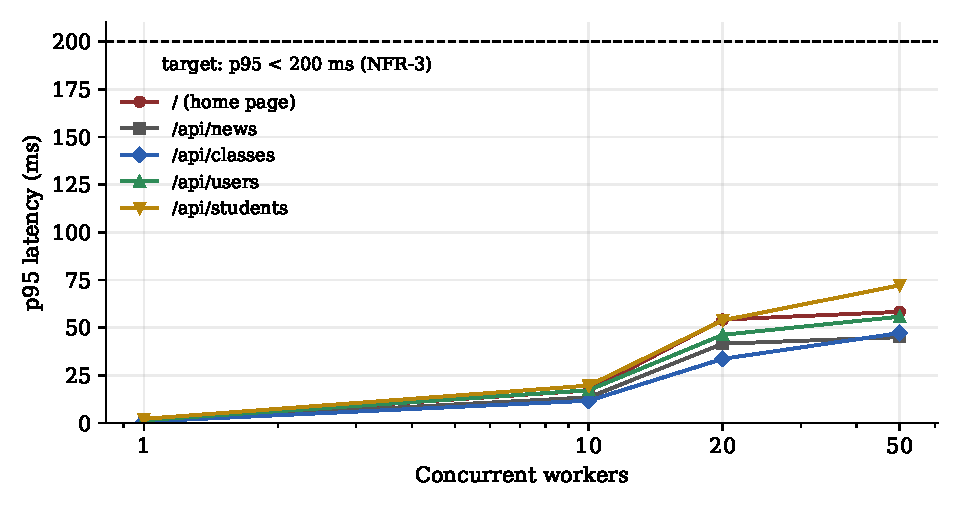
\includegraphics[width=0.82\textwidth]{fig/load_p95.pdf}
\caption{95th-percentile latency against the number of concurrent workers}
\label{fig:load}
\end{figure}

The result supports the stated requirement for this data size and configuration. It does not establish capacity for a larger school, for a database on separate hardware, for write-heavy periods such as the end of a term, or for repeated runs: each level was run once, so there is no estimate of run-to-run variation.

\section{Browser and interface checks}
\label{sec:ui}

The browser test (Playwright with Chromium) creates its own data through the administrator API and then walks through the main journeys: the guest sees the home page; an administrator publishes a news item whose title contains HTML tags, and the page shows the tags as text without interpreting them; a teacher gives a mark in the gradebook; a pupil opens the dashboard and the marks page; a pupil receives 403 when requesting an administrator page; a pupil downloads a CSV file; and the home page at phone width does not scroll horizontally. The test passed.

In addition, the main pages of the five kinds of user (guest, pupil, parent, teacher, administrator) were opened in a browser and the network and console were observed: 16 page loads produced no response with status 400 or higher and no console error. At a viewport of 390\,px the document width equalled the viewport width, so there was no horizontal overflow. These are functional checks; they are not an accessibility audit, and contrast, keyboard operation and screen-reader behaviour were not formally evaluated.

\section{Security checks}

Table~\ref{tab:security} lists the security behaviour that is covered by automated tests and by observation. The login limiter was also seen in operation during the load and browser runs: after more than ten sign-ins within a minute from one address the server answered 429 until the window expired, which had to be worked around by restarting the server with a higher limit for the repeated tests.

\begin{table}[H]
\centering
\caption{Security behaviour and how it was checked}
\label{tab:security}
\small
\begin{tabularx}{\textwidth}{@{}>{\raggedright\arraybackslash}p{4.3cm}X@{}}
\toprule
Mechanism & Check \\
\midrule
Closed registration & Public registration request returns 401; accounts exist only after administrator action \\
Role boundaries & Pupil cannot read another pupil; parent limited to linked children; pupil receives 403 on administrator pages \\
CSRF & State-changing web request without a matching \code{Origin} or \code{Referer} receives 403 \\
Cookie flags & Session cookie is \code{HttpOnly} and \code{SameSite=Strict} \\
Script injection & News title and text with HTML are displayed as text (unit scenario and browser test) \\
CSV formula injection & Cells starting with \code{=}, \code{+}, \code{-} or \code{@} are prefixed in the export test \\
Response headers & Content-security policy, frame and content-type options present on responses \\
Login limit & Eleventh attempt within a minute returns 429 with \code{Retry-After} \\
\bottomrule
\end{tabularx}
\end{table}

\section{Defects found during final verification}

The final verification also found three problems, which were corrected. First, the news feed card showed only the first paragraph of an item, so a pinned announcement that began with a one-line greeting looked empty; the preview now collapses the whole text and a test covers it. Second, the continuous-integration definition in the repository still described the earlier test set and PostgreSQL 15; it was rewritten to use PostgreSQL 16 and to run the HTTP scenarios on a clean database, a backup and restore round trip, a short load test and the browser test. Third, the PostgreSQL scenario failed on a database that already contained an administrator, because it relied on the start-up bootstrap, which does nothing in that case. It now creates its own administrator directly in the repository; the corrected scenario passed on three databases, among them one with the demonstration data and one with the load-test data.

\section{Assessment and limitations}
\label{sec:limits}

The evaluation supports the intended workflow: marks on the five-point scale are validated at three levels and aggregated by a stated rule; the weekly diary and the home page work for all roles; and the response-time requirement is met on a school-sized data set. The results are limited in the following ways.

\begin{itemize}
  \item \textbf{No user study.} The usability test plan (five participants per role group, think-aloud tasks, task success and the System Usability Scale \cite{sus}) is prepared but was not carried out. Claims about ease of use, and the resemblance of the interface to the diary services that inspired it, rest on design reasoning and on the automated checks, not on user data.
  \item \textbf{Performance scope.} The load figures come from one shared two-core virtual machine, one run per level, with the load generator on the same host. They do not predict behaviour under larger data, separate hardware or write-heavy load.
  \item \textbf{Toolchain.} Tests were run with Go 1.24.7, while the module file and the container image target Go 1.21 and the pipeline pins that version. The compiler enforces the language level of the module file, and a search of the sources found none of the standard-library additions made after Go 1.21 that could be checked by name, but no build with a 1.21 toolchain was made here. The pipeline is the authority for compatibility with the older toolchain.
  \item \textbf{Coverage.} The page-handler layer is covered mostly by the browser test rather than by Go tests, and repository code is exercised only when the PostgreSQL scenarios run.
  \item \textbf{Deployment model.} The reminder job and the login limiter keep state in one process. Several instances would need shared scheduling and a shared limiter, and a reverse proxy must pass the client address correctly for the limiter to see individual clients.
  \item \textbf{Interface.} The interface is English only, news is plain text without formatting or attachments, and there is no accessibility audit.
  \item \textbf{Data conversion.} The conversion of legacy 0--100 scores to marks is lossy and irreversible in practice. It is appropriate for a demonstration database; a school with real historical scores would have to agree the bands with its teachers first.
\end{itemize}
